\pagenumbering{arabic}

\chapter{Introduction} \label{introduction}
This document is the Software Specification Requirement (SRS) of an open source system called FarmBot \cite{FarmBotWhitepaper}. The system has a website \cite{FarmBotWebsite} and a GitHub repository \cite{FarmBotGitHub}.

\section{Purpose of the System }
FarmBot is designed to integrate the advantages of both monocrop and polycrop agriculture systems, aiming to maximize the benefits while minimizing the drawbacks of each. Monocropping is highly efficient from a machinery perspective, which allows for large-scale operations with minimal human labor due to its simplicity and reliance on a single plant species. However, it lacks biological efficiency because it requires extensive inputs like fertilizers, pesticides, and water, and is prone to environmental issues such as topsoil depletion and groundwater pollution. Polycropping, on the other hand, excels in biological efficiency by enhancing ecosystem diversity, which reduces the need for external inputs and creates a more stable and sustainable farming system. Yet, it falls short in machine efficiency. It requires more human labor due to the absence of suitable equipment for managing diverse crops.\\\\
FarmBot addresses these challenges by being a scalable farming equipment that can manage a polycrop with similar machine efficiency and minimal labor requirements associated with the monocrop agriculture system. The main purpose of FarmBot is to establish farms that are abundant, resilient, sustainable, and efficient by leveraging the strengths of both monocrop and polycrop systems.
\section{Scope}
FarmBot aims to modernize agriculture by automation, and it helps to apply both individual and commercial farming operations requiring efficiency, sustainability, and scalability. The project will deliver FarmBot's integrated software package, an open-source cloud-based Software as a Service (SaaS) solution. \\\\
FarmBot offers a bunch of key benefits aimed at transforming modern agriculture: it boosts crop yields, minimizes waste of resources, and improves operational efficiency. This software is designed to generalize precision farming, making it accessible to a wider audience by harnessing technology for sustainable agricultural practices. The goals of the FarmBot project are to make advanced farming technology more universally applicable, support data-driven agricultural methods, and inspire society to adopt cutting-edge agricultural systems. The development and features of the FarmBot software are rigorously crafted to support these objectives, which ensure a direct contribution to enhancing agricultural productivity and sustainability through technological advancement. Some components of the software are:

\begin{itemize}
    \item A user-friendly web frontend which enable users to design and plan farm layouts.
    \item Decision support system which includes data mapping and analysis tools that helps the user to store, access, and analyze farming data, thus, utilize analytics for optimizing farming operations.
    \item User, farm, and equipment profile management systems. By means of user profiles, work and data of the user can be saved and later accessed. Also, user profiles provide authentication against the hacking purposes. Farm profiles include the data associated with the farm including plant layouts, scheduled operations, statistics, and history of the farm. Via the equipment profiles, information about equipments is stored and easily modified as equipment is upgraded or become inactive for maintenance.
    \item Microcontroller software for direct hardware interaction that helps the user to control FarmBot hardware.
    \item Open data repositories for community-driven knowledge sharing.
\end{itemize}

\section{System Overview}
\subsection{System Perspective}
FarmBot operates as an autonomous system that integrates with various services for comprehensive farm management. Users engage with the Web Application to design their farms and issue commands, which are sent to FarmBot for execution. The system captures a variety of farm-related data including logs, sensor readings, and visual documentation of the farm. For a broader scope of agricultural data, the Web Application interfaces with the OpenFarm.cc API, enriching the user's resources for crop management. Internally, FarmBot utilizes a Raspberry Pi Controller, communicating through MQTT protocol, to manage operations and collect data. This controller then issues precise operational commands to the Arduino Firmware, which engages with an array of sensors and tools to perform essential farming tasks such as seeding, watering, and monitoring environmental conditions. The system admin plays a vital role in maintaining the software's operational integrity, while the farm itself is the physical space where FarmBot's tools are deployed. The simplicity of the user experience is thanks to the sophisticated backend processes that enable seamless operation and real-time data exchange, ensuring that the user remains at the forefront of the agricultural management experience.

\newpage

\begin{figure}[htbp]
    \centering
    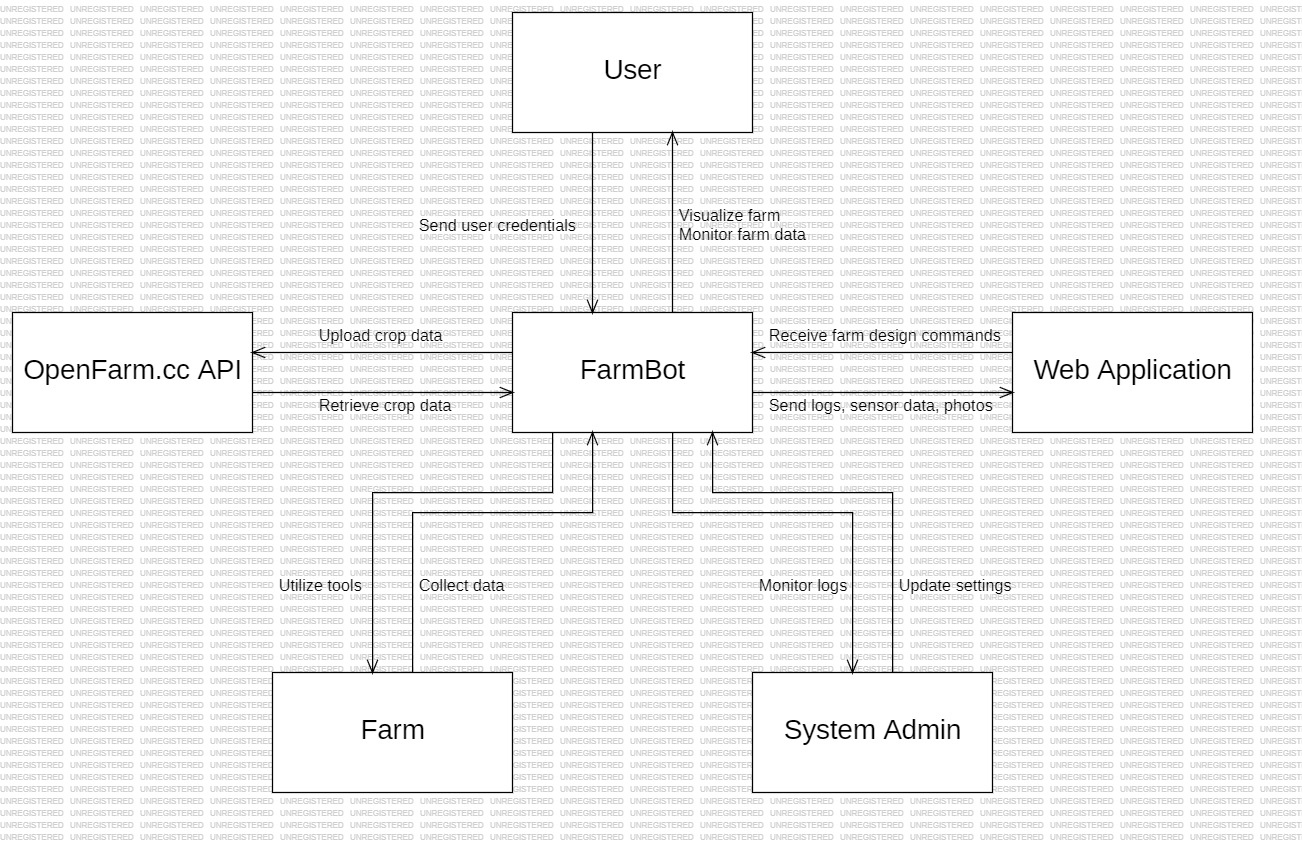
\includegraphics[width=1\linewidth]{Figures/context_diagram.jpg}
    \caption{System Context Diagram}
    \label{System Context Diagram}
\end{figure}

\subsubsection{System Interfaces}
\begin{itemize}
    \item \textbf{Decision Support System:} The Decision Support System within FarmBot is a key algorithmic component designed to optimize farm management through data-driven decisions. It analyzes various data streams, such as weather patterns and soil properties, to determine the best settings for farming operations like seed spacing, watering, and planting schedules. A high-level overview in Figure \ref{Decision Support System} shows the Decision Support System combining data streams to make informed decisions for each FarmBot operation, significantly enhancing efficiency and productivity in farm management.

    \begin{figure}[htbp]
        \centering
        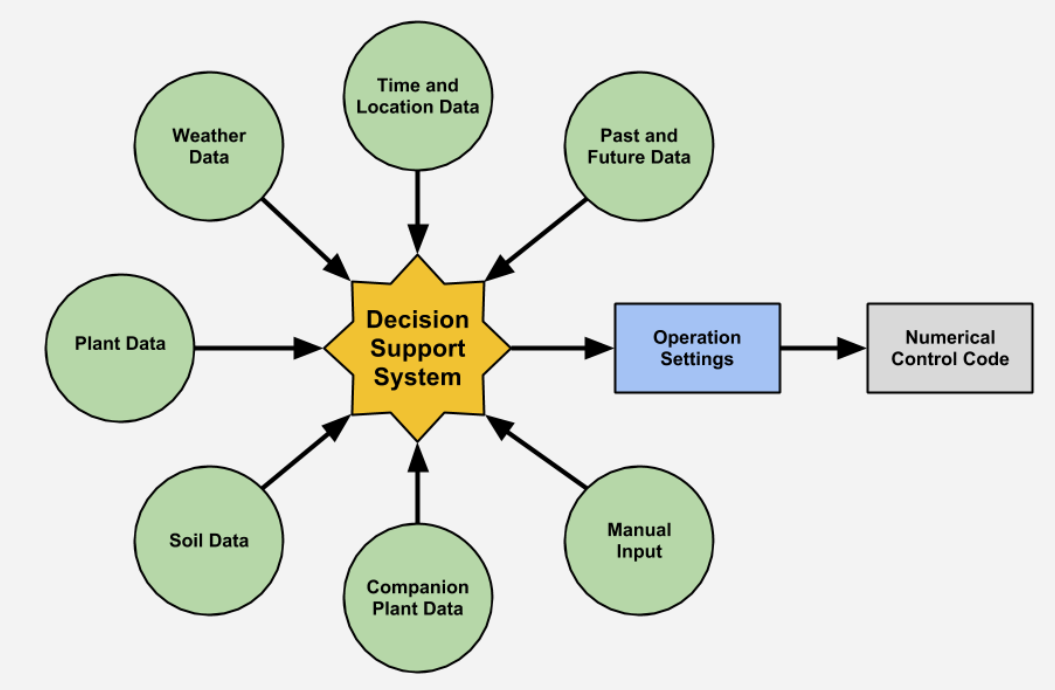
\includegraphics[width=1\linewidth]{Figures/dss.png}
        \caption{Decision Support System}
        \label{Decision Support System}
    \end{figure}
    
    \item \textbf{Data Management System:} Data Management System is a critical interface in FarmBot, focusing on the collection, storage, and utilization of diverse data types on an SQL database to optimize farming practices. Key components include:
    \begin{itemize}
        \item \textbf{Plant Data:} Covers specifics like sun requirements, seed spacing, and watering needs for optimal growth conditions.
        \item \textbf{Soil Data:} Involves systematic collection of soil characteristics (moisture, nutrients, composition) for precise soil management.
        \item \textbf{Companion Plant Data:} Uses information on plant relationships to maximize polycropping benefits, such as pest control and nitrogen fixation.
        \item \textbf{Time and Location Data:} Enables FarmBot to perform operations based on current time and geographical positioning, optimizing planting and watering schedules.
        \item \textbf{Weather Data:} Integrates forecasts to make informed decisions on watering and protects crops from adverse weather conditions.
        \item \textbf{Topography:} Assists in plant placement and water flow management by analyzing land contours and sunlight exposure.
        \item \textbf{Past and Future Data:} Utilizes historical farm data and future plans for crop rotation and soil improvement strategies.
        \item \textbf{Manual Input Data:} Allows for the customization of farming operations based on farmer knowledge and unique environmental factors.
    \end{itemize}
        
    \item \textbf{RESTful JSON API:} The FarmBot WebApp uses RESTful JSON API, crucial for enabling efficient communication across the software's various components. This API plays a pivotal role in managing data flow, including user account details, farm designs, sequences, authorization tokens, and other essential resources. By leveraging JSON for data formatting, the API ensures streamlined and lightweight data exchange, enhancing web application performance. This RESTful approach facilitates a dynamic and interactive user experience, allowing for seamless operation and customization of the FarmBot system. The API's design, rooted in open-source and cloud-based technologies, supports the flexible and accessible management of automated farming operations, making it a fundamental element of the FarmBot WebApp's infrastructure.

    \item \textbf{Webcam:} The webcam interface in FarmBot captures images of the farm, allowing for visual monitoring and progress tracking. These photographs are sent to the Raspberry Pi microcontroller, providing users with up-to-date visual data accessible via the FarmBot WebApp, aiding in both immediate and long-term farm management and planning.

\end{itemize}

\subsubsection{User Interfaces}
The FarmBot WebApp's user interface is designed to be engaging, intuitive, and efficient. It allows users straightforward access to all software functionalities. The interface employs a tabbed layout, with each tab featuring multiple panes for specific user actions and needs.

\begin{itemize}
    \item \textbf{Register \& Login Tab:} The Register \& Login Tab serves as the entry point to the FarmBot WebApp, requiring users to authenticate via email and password, as shown on the Figure \ref{Register Login Tab}.\\

    \begin{figure}[htbp]
        \centering
        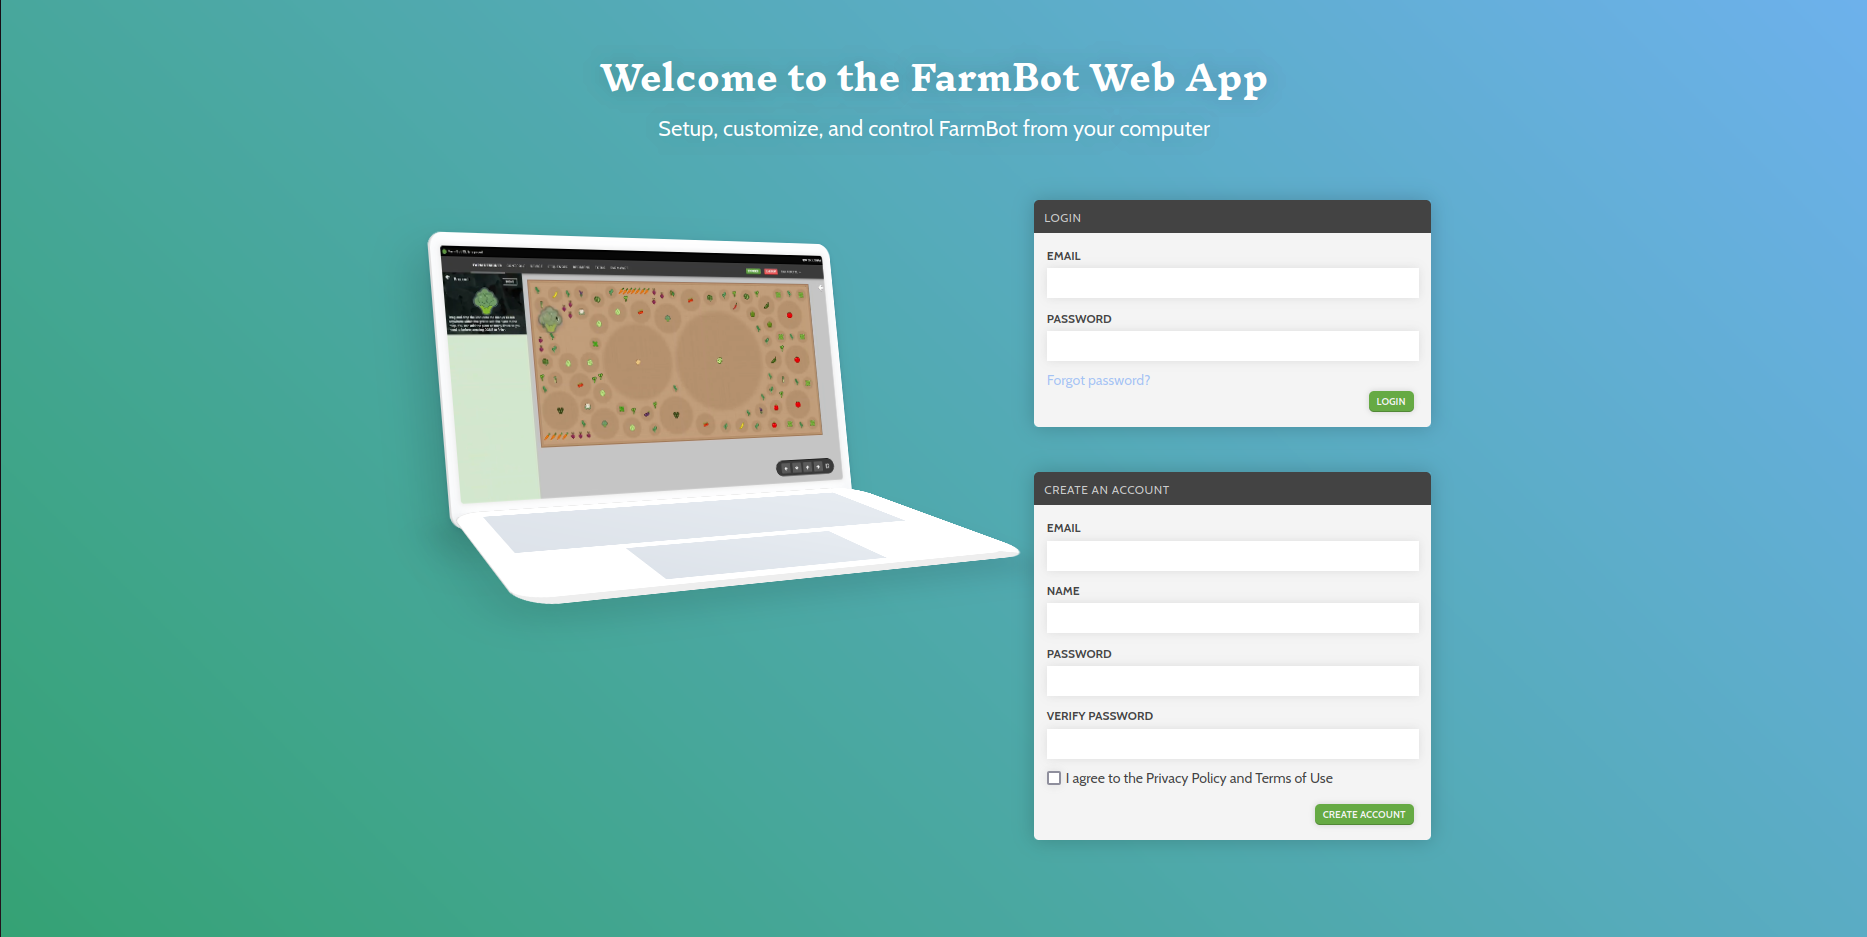
\includegraphics[width=1\linewidth]{Figures/register_login_tab.png}
        \caption{Register \& Login Tab}
        \label{Register Login Tab}
    \end{figure}
    
    \item \textbf{Dashboard Tab:} Overview of this tab can be seen in Figure \ref{Dashboard Tab}. This tab provides a comprehensive overview of the FarmBot system's operations and statistics, divided into various panes for detailed insights:
    \begin{itemize}
        \item \textbf{Hardware Information Pane:} Users can select and manage hardware components through dropdown menus, enabling easy configuration of the FarmBot system's physical setup.
        \item \textbf{Resource Usage Pane:} An interactive graph displays the consumption of resources (electricity, water, seeds, etc.) over time, with breakdowns and cost analysis based on user input.
        \item \textbf{System Information and Control Pane:} Displays general system information and manual control options for immediate adjustments.
        \item \textbf{Financial Analysis Pane:} Presents an overview of the operation's financial aspects, including cost and revenue projections.
    \end{itemize}
 
    \begin{figure}[htbp]
        \centering
        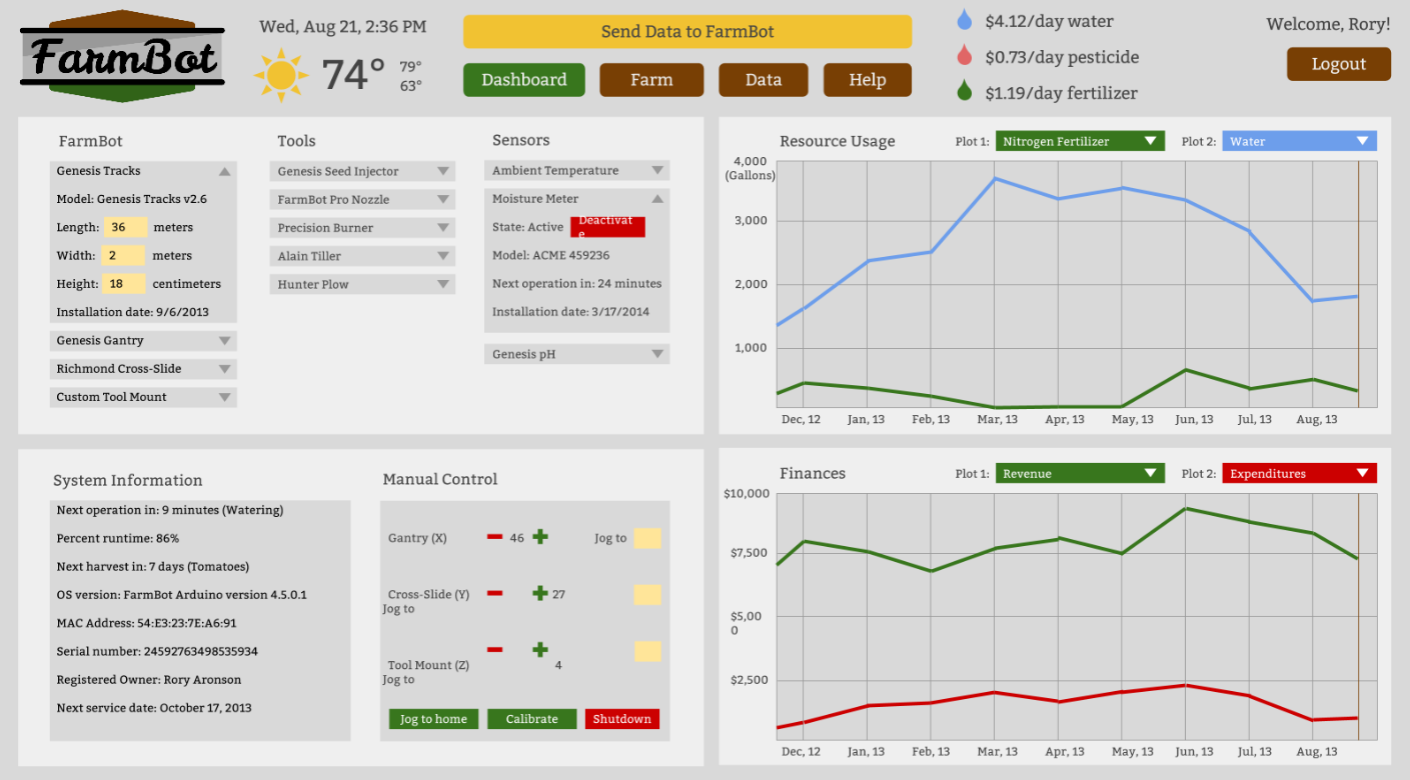
\includegraphics[width=1\linewidth]{Figures/dashboard_tab.png}
        \caption{Dashboard Tab}
        \label{Dashboard Tab}
    \end{figure}
    
    \item \textbf{Farm Tab:} The Farm Tab, which can be seen in Figure \ref{Farm Tab}, is central to planning and executing farming operations, consisting of three main sections:
    \begin{itemize}
        \item \textbf{Plants and Operations Toolbox:} Enables users to select and customize plantings and operations.
        \item \textbf{Farm Map:} An interactive, zoomable map of the farm layout where users can arrange and modify plantings and operations.
        \item \textbf{Operations Agenda:} Lists scheduled operations with a calendar view, allowing users to plan and adjust farming activities.
    \end{itemize}
 
    \begin{figure}[htbp]
        \centering
        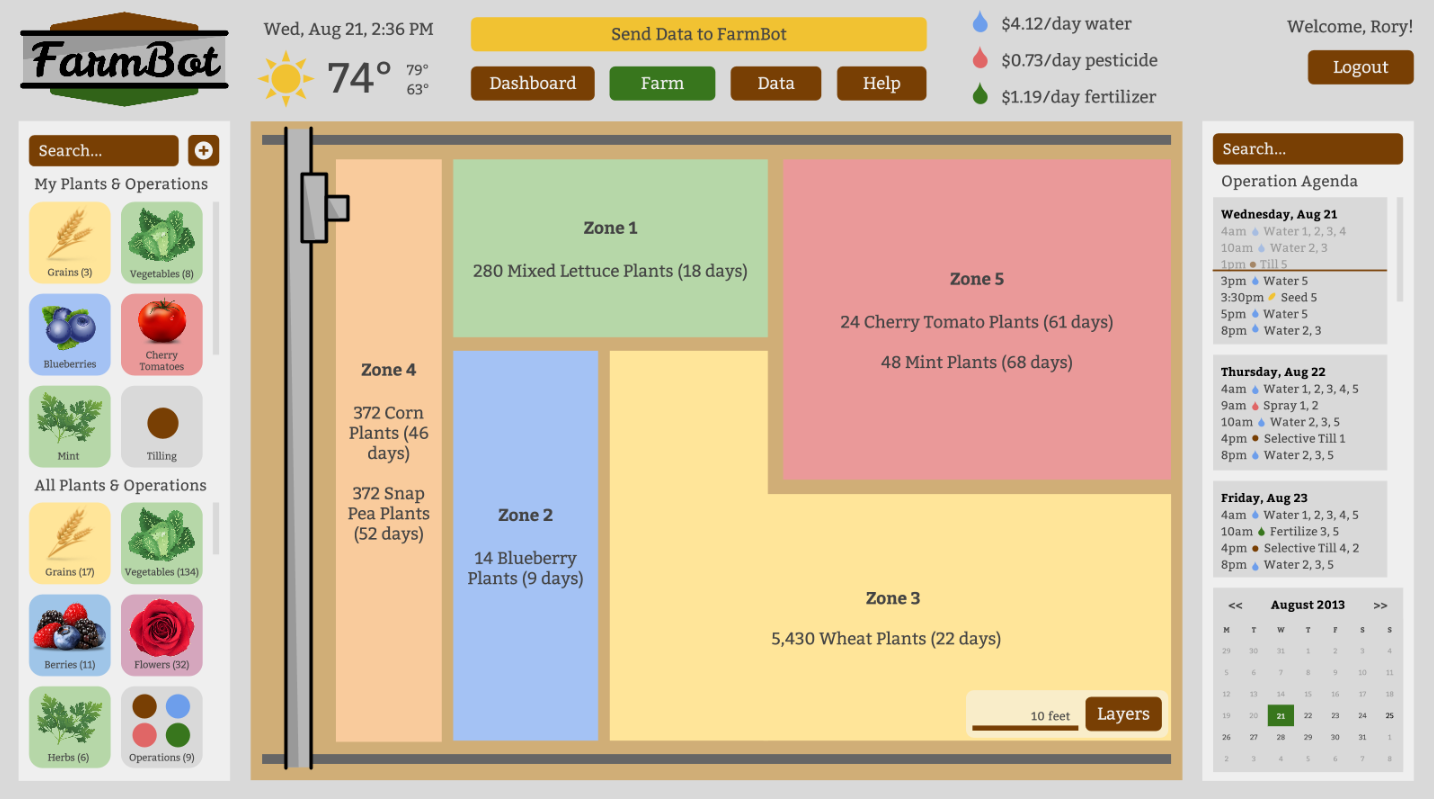
\includegraphics[width=1\linewidth]{Figures/farm_tab.png}
        \caption{Farm Tab}
        \label{Farm Tab}
    \end{figure}
    
    \item \textbf{Data Tab:} Utilizes FarmBot hardware for detailed data collection. Enables the creation of data maps that inform decision-making processes. These maps highlight areas needing adjustments (e.g., watering, soil amendments) and provide insights into soil moisture, temperature, and other critical factors.
    
\end{itemize}

\subsubsection{Hardware Interfaces}
\begin{itemize}
    \item \textbf{Microcontrollers}
    \begin{itemize}
        \item \textbf{Raspberry Pi:} The Raspberry Pi acts as the brain of the FarmBot system, handling lightweight processes generated by the Decision Support System. It communicates with the Arduino to send G-Codes and F-Codes for the execution of various operations and receives feedback on the operations performed.
        \item \textbf{Arduino:} The Arduino microcontroller is tasked with receiving G-Codes and F-Codes from the Raspberry Pi, executing these commands, and reporting the outcomes back to the Raspberry Pi. It directly controls the mechanical components of the FarmBot for precise operation execution.
    \end{itemize}

    \item \textbf{Other Hardware Interfaces}\\
    FarmBot's hardware closely resembles that of 3D printers and CNC milling machines, comprising components like tracks, gantry, cross-slide, and tool mounts that facilitate movement and operation execution in three dimensions (X, Y, and Z). Hardware overview can be seen in Figure \ref{Hardware Overview}. The system's design allows for scalability in all dimensions, ensuring FarmBot's adaptability to various farm sizes and operational needs. Key hardware components include:
    \begin{itemize}
        \item \textbf{Tracks:} Fixed rails that provide precision and support for the gantry, allowing for highly accurate positioning.
        \item \textbf{Gantry:} Bridges the tracks and moves along the X-direction, serving as a base for the Y-direction movement of the cross-slide and Z-direction movement of the tool mounts.
        \item \textbf{Cross-Slide:} Moves across the gantry in the Y-direction, enabling the FarmBot to perform operations anywhere within the XY plane.
        \item \textbf{Tool Mounts:} Attached to the cross-slide, facilitates Z-direction movement and serves as the point of attachment for various tools required for farming operations.
        \item \textbf{Tools:} Customized agricultural tools adapted for use with FarmBot, including seed injectors, watering nozzles, sensors, and plows, among others.
        \item \textbf{Electronics:} Comprise motors, servos, solenoids, valves, and sensors controlled by the microcontrollers, essential for the operation of FarmBot.
        \item \textbf{Sensors:} Utilized for data collection to inform decisions about farm setup and operations, enhancing the "Smart Farming" capabilities of FarmBot.
    \end{itemize}
\end{itemize}

\begin{figure}[htbp]
        \centering
        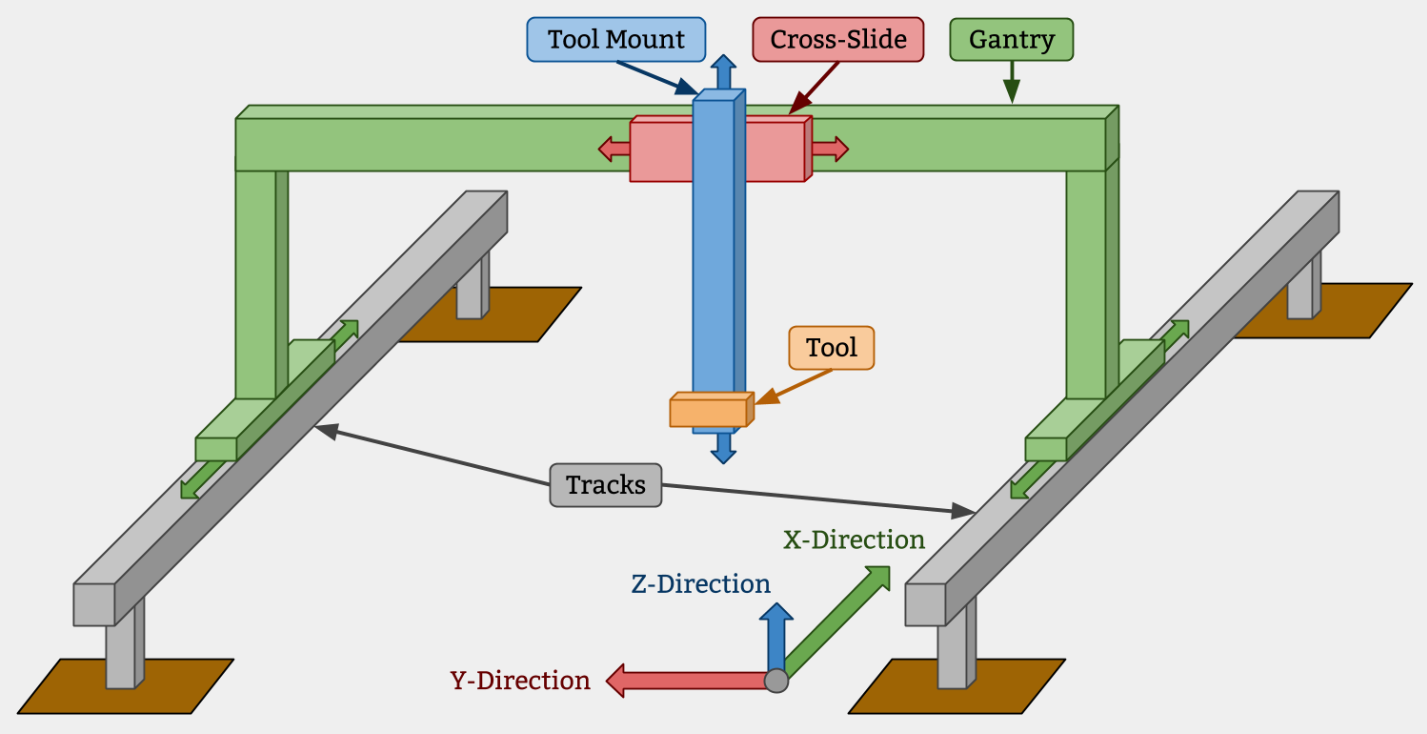
\includegraphics[width=1\linewidth]{Figures/hardware.png}
        \caption{Hardware Overview}
        \label{Hardware Overview}
\end{figure}

\subsubsection{Software Interfaces}
\begin{itemize}
    \item \textbf{FarmBot WebApp:} Provides a central interface for users to manage and program their FarmBot. It includes a RESTful JSON API for data management and a Dockerized MQTT server for real-time device communication. The web app is designed with a tabbed interface for easy navigation, allowing users to oversee FarmBot operations, design farm layouts, and analyze data through interactive maps and panels.
    \item \textbf{FarmBot OS:} Custom-designed for the Raspberry Pi, facilitates communication and operation capabilities. It connects with the web application via hosted MQTT gateway for synchronization tasks, including downloading sequences and farm designs, and uploading logs and sensor data. Additionally, it handles real-time commands, and sends them to the Arduino for command execution and data collection, and manages images with compatibility for USB or Raspberry Pi cameras.
    \item \textbf{Microcontroller Software:} Embedded within FarmBot's hardware, the microcontroller software interprets numerical codes from the backend, manages hardware operations like sensor readings and motor movements, and communicates real-time data back to the cloud. Optimized for efficiency, it conducts complex computational tasks remotely, relying on cloud-based decision support systems to process data and send simplified operational instructions to FarmBot, similar to the G-code used in CNC machining and 3D printing. This setup emphasizes a division of labor, with heavy processing offloaded to the cloud and the microcontroller focusing on direct hardware control.
\end{itemize}

\subsubsection{Communication Interfaces}
The communication interfaces of FarmBot facilitate secure and efficient interaction between the user, the FarmBot WebApp, and the FarmBot hardware, utilizing:
\begin{itemize}
    \item \textbf{RPC:} This mechanism is primarily employed for user authentication, enabling secure connections to the FarmBot WebApp. It allows the system to perform actions on behalf of the user after verifying their identity, ensuring that only authorized users can access and control the FarmBot operations.
    \item \textbf{HTTP/HTTPS:} The backbone of communication within the FarmBot WebApp, HTTP/HTTPS is utilized for all web-based interactions. HTTPS, the secure version of HTTP, ensures that data transferred between the user's browser and the FarmBot WebApp is encrypted, providing a protected channel for the transmission of sensitive information such as user account details, farm designs, and operational data.
    \item \textbf{MQTT:} MQTT in FarmBot enables real-time messaging between the web application and Raspberry Pi microcontroller, crucial for immediate command execution and data exchange. WebApp uses MQTT, a lightweight protocol ideal for IoT communications, managed through a broker for efficient message distribution.
    \item \textbf{WiFi:} A link for configuring the FarmBot system, WiFi enables the transmission of user credentials to the FarmBot Configurator. This interface is essential for initializing communication between the user and the Raspberry Pi, setting up the device with the necessary access permissions for operation.
    \item \textbf{USB:} The USB interface in FarmBot enables data transfer between the Arduino and Raspberry Pi, essential for synchronized operations and task execution. This direct connection via USB ports ensures continuous communication, critical for the system's precision and functionality.
    \item \textbf{Ethernet:} The Ethernet port on the Raspberry Pi provides an optional wired network connection for FarmBot, offering an alternative to WiFi. This feature allows users to prefer a more stable and secure connection, accommodating environments where WiFi reliability may be a concern, thus enhancing the system's connectivity flexibility.
\end{itemize}

\subsubsection{Memory Constraints}
Since the FarmBot application is cloud-based, it does not face any significant memory constraints. The extensive farm data is managed and stored on the cloud, ensuring that the system's performance remains unaffected by the volume of data. This setup allows for scalability and efficient data handling without burdening local resources.

\subsubsection{Operations}
FarmBot operations can be divided into:
\begin{itemize}
    \item \textbf{User Operations:}
    \begin{itemize}
        \item Design farm layouts
        \item Schedule tasks
        \item Send manual control commands
        \item Observe logs, sensor data and photos
        \item Monitor performance
    \end{itemize}
    \item \textbf{System Operations:}
    \begin{itemize}
        \item Automatically execute scheduled tasks
        \item Regularly backup data such as user accounts, farm designs, and operational histories
        \item Recover data in the case of system failures
    \end{itemize}
\end{itemize}

\subsection{System Functions}
\begin{longtblr}
[
 caption = {System Functions},
 label = {System Functions}
]
{
  colspec = {|X|X|},
  hlines
}

\textbf{Function} & \textbf{Summary} \\ \hline
Design Farm Layouts & Users can create and modify the spatial arrangement of crops and infrastructure on their digital farm using the WebApp.\\ \hline
Schedule Tasks & Users have the capability to plan and set specific times for FarmBot to perform agricultural activities such as planting, watering, and harvesting.\\ \hline
Send Manual Control Commands & This operation allows users to directly command FarmBot to perform immediate actions, bypassing automated schedules for tasks like troubleshooting or specific, non-routine interventions.\\ \hline
Observe Logs, Sensor Data, and Photos & Users can access detailed records of FarmBot's operations, environmental sensor readings, and visual documentation captured by the device, enabling monitoring and decision-making based on real-time and historical data.\\ \hline
Monitor Performance & This involves users tracking the effectiveness and efficiency of FarmBot's operations over time, including its adherence to schedules and the success rate of completed tasks.\\ \hline
Automatically Execute Scheduled Tasks & FarmBot autonomously carries out agricultural operations based on the schedules set by the user, operating independently from the user during these periods.\\ \hline
Regularly Backup Data & The system periodically saves copies of crucial data such as user accounts, farm designs, and logs of operational history to cloud storage, safeguarding against data loss.\\ \hline
Recover Data in Case of System Failures & In the event of hardware or software malfunctions, the system can restore previously backed-up data to return to normal operations with minimal disruption.
\end{longtblr}

\subsection{Stakeholder Characteristics}
The FarmBot project serves diverse user categories, including hobbyist gardeners, professional farmers, educators, and researchers.
\begin{itemize}
    \item \textbf{Hobbyist gardeners and professional farmers:} Primarily use FarmBot for its automated farming capabilities, requiring minimal technical skills thanks to its user-friendly interface.
    \item \textbf{Educators:} Employ FarmBot as a practical tool to demonstrate the integration of technology in agriculture, necessitating a good understanding of the system for effective teaching.
    \item \textbf{Researchers:} Focus on using FarmBot for studies in sustainable farming and crop optimization. They need to have a strong background in agricultural science and research methodologies.
\end{itemize}

\subsection{Limitations}
\begin{itemize}
    \item \textbf{Regulatory Policies:} FarmBot is an open source hardware and software project. Therefore the project files and codes are accessible for everyone.
    \item \textbf{Hardware Limitations:} The precision and efficiency of FarmBot are dependent on the performance of its hardware components, such as motors, sensors, and microcontrollers. These components must function without delay to maintain operational accuracy and reliability.
    \item \textbf{Interfaces to Other Applications:} FarmBot's functionality is enhanced through compatibility with various software applications, including cloud-based services and data analytics tools.
    \item \textbf{Parallel Operation:} FarmBot is designed to perform multiple operations simultaneously, such as watering and collecting the sensor data. This requires robust system design to manage concurrent tasks effectively.
    \item \textbf{Audit Functions:} While FarmBot collects extensive operational data, its audit capabilities are designed to focus on system performance and user actions, potentially limiting comprehensive auditing of all system interactions.
    \item \textbf{Control Functions:} FarmBot relies on both automated sequences and user-initiated commands for operation.
    \item \textbf{Higher-order Language Requirements:} The system's software is developed using high-level programming languages, such as TypeScript, Ruby, Elixir, Python, and C++. This ensures ease of maintenance, updates, and scalability.
    \item \textbf{Signal Handshake Protocols:} Communication between FarmBot's components, including the Raspberry Pi and Arduino microcontrollers, or web app and hardware utilizes protocols to ensure data integrity and synchronization.
    \item \textbf{Quality Requirements:} The reliability and durability of FarmBot are critical. The system meets agricultural productivity and efficiency standards.
    \item \textbf{Criticality of the Application:} The FarmBot is not a critical system. It will not cause any huge impact if it fails.
    \item \textbf{Safety and Security Considerations:} Given its internet connectivity, FarmBot contains security measures to protect user data and system integrity, although being open-source may expose it to potential vulnerabilities that require ongoing attention.
    \item \textbf{Physical/Mental Considerations:} FarmBot is designed to be accessible to users with varying levels of physical ability and technical expertise.
    \item \textbf{Limitations from Other Systems:} FarmBot's performance and capabilities may be influenced by the limitations of integrated systems and platforms, including real-time data processing and cloud storage services.
\end{itemize}

\newpage
\section{Definitions}
\begin{longtblr}
[
 caption = {Definitions},
 label = {Definitions}
]
{
  colspec = {|X|X|},
  hlines
}
SRS & A software requirements specification (SRS) is a description of a software system to be developed. \\ \hline
SaaS & Software as a service (SaaS) is a software licensing and delivery model in which software is licensed on a subscription basis and is centrally hosted. \\ \hline
MQTT & Message Queue Telemetry Transport (MQTT) is a lightweight, publish-subscribe, machine to machine network protocol for message queue/message queuing service. \\ \hline
WiFi & Wireless Fidelity (WiFi) is a family of wireless network protocols based on the IEEE 802.11 family of standards, which are commonly used for local area networking of devices and Internet access, allowing nearby digital devices to exchange data by radio waves. \\ \hline
G-Code & Geometry code (G-code) is the most widely used computer numerical control (CNC) and 3D printing programming language. \\ \hline
WebApp & A web application (web app) is application software that is accessed using a web browser. Web applications are delivered on the World Wide Web to users with an active network connection. \\ \hline
DSS & A decision support system (DSS) is an information system that supports business or organizational decision-making activities. \\ \hline
SQL & Structured Query Language (SQL) is a domain-specific language used to manage data, especially in a relational database management system (RDBMS). \\ \hline
REST & Representational State Transfer (REST) is a software architectural style that was created to guide the design and development of the architecture for the World Wide Web. \\ \hline
JSON & JavaScript Object Notation (JSON) is an open standard file format and data interchange format that uses human-readable text to store and transmit data objects consisting of attribute–value pairs and arrays (or other serializable values). \\ \hline
API & An application programming interface (API) is a way for two or more computer programs or components to communicate with each other. \\ \hline
CNC & Computer Numerical Control (CNC) is the automated control of tools by means of a computer. It is used to operate tools such as drills, lathes, mills, grinders, routers and 3D printers. \\ \hline
USB & Universal Serial Bus (USB) is an industry standard that allows data exchange and delivery of power between many various types of electronics. \\ \hline
RPC & In distributed computing, a remote procedure call (RPC) is when a computer program causes a procedure (subroutine) to execute in a different address space (commonly on another computer on a shared network), which is written as if it were a normal (local) procedure call, without the programmer explicitly writing the details for the remote interaction. \\ \hline
HTTP & The Hypertext Transfer Protocol (HTTP) is an application layer protocol in the Internet protocol suite model for distributed, collaborative, hypermedia information systems. \\ \hline
HTTPS & Hypertext Transfer Protocol Secure (HTTPS) is an extension of the Hypertext Transfer Protocol (HTTP), and it uses encryption for secure communication over a computer network, and is widely used on the Internet. \\ \hline
IoT & The Internet of things (IoT) describes devices with sensors, processing ability, software and other technologies that connect and exchange data with other devices and systems over the Internet or other communications networks.
\end{longtblr}
